\subsection{ADC-PCB "Prototype 1"} \label{Prototype1}
\subsubsection{Projektteilbereich Übersicht}
Zum Testen und erstmaligen Ansteuern des extrernen ADCs (siehe: \ref{extADC}) wurde ein extra PCB angefertigt. Der Schaltplan und das Platinenlayout wurden in KiCad gezeichnet, die Gerberdateien exportiert und die Platine anschließend mithilfe einer CNC-Fräsmaschiene gefertigt. Das Löten von sehr kleinen SMD-Bauteilen war neu für uns und wir freuten uns das dazuzulernen. Unterstützung bekam die Projektgruppe von Prof. Graupe. 

\subsubsection{Schaltplan}
Der Schaltplan (Figure: \ref{Prot1_Schalt}) wurde möglist simpel gehalten, es befindet sich ausschließlich der ADC mit seinen obligatorischen Stützkondensatoren auf der Platine und Pinheader zum Anschließen, sowie ein Eingangswiderstand für den Analogeingang. Die Spannungsversorgung als auch die Kommunikation erfolgen über die Pinheader zum FPGA. Der Verwendete ADC ist ein LTC1420C (siehe: \ref{LTC1420C}).
\begin{figure}[h!]
\begin{center}
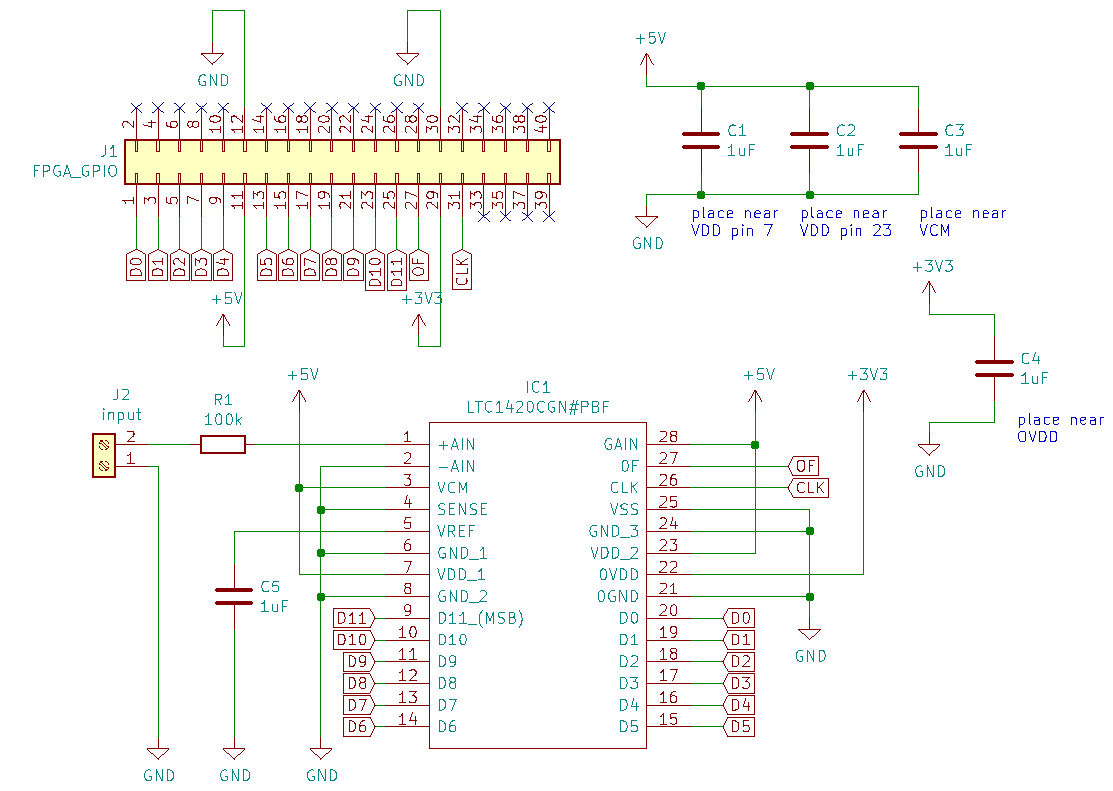
\includegraphics[width = 15cm]{SAUER/Grafiken/Prot1/Prot1_Schalt.png}
\caption{Schaltplan "Prototype 1"}
\label{Prot1_Schalt}
\end{center}
\end{figure}

\subsubsection{PCB}
Das Platinenlayout ist einseitig ausgeführt, möglichst simpel und klein gehalten. Über 2x20 Pinheader wird das Board auf das FPGA gesteckt und sosowohl elektrisch als auch mechanisch verbunden. Die Platine hat die Maße 54,6 x 23,5 mm, wie in Figure \ref{Prot1_BFAB} ersichtlich. Die Nähe der Clock-Leitung zu der Leitung für das analoge Eingangssignal ist sehr unvorteilhaft, jedoch für die Kommunikation zwischen FPGA und ADC irrelevant.
\begin{figure}[H]
\begin{center}
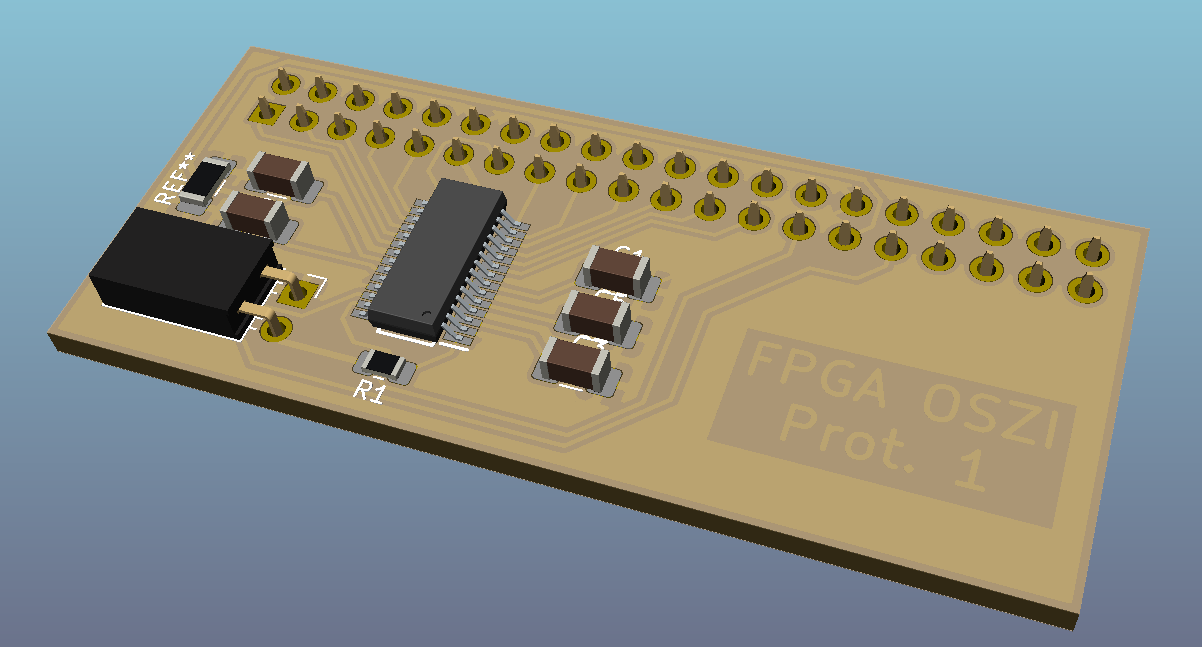
\includegraphics[width = 15cm]{SAUER/Grafiken/Prot1/3DF.png}
\caption{3D-Ansicht Vorderseite}
\end{center}
\end{figure}

\begin{figure}[H]
\begin{center}
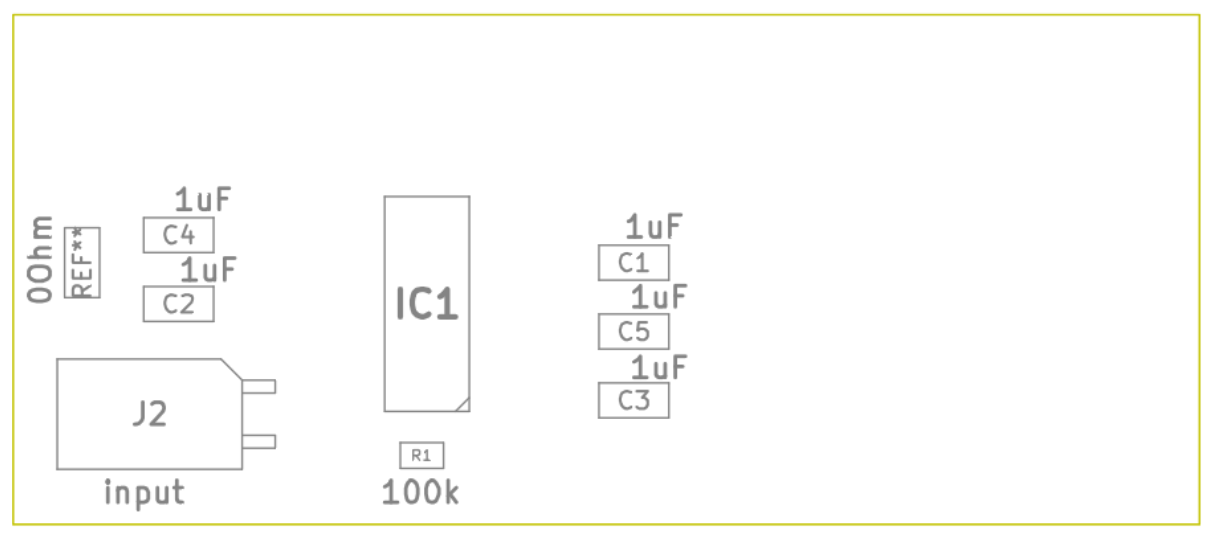
\includegraphics[width = 15cm]{SAUER/Grafiken/Prot1/FFAB.png}
\caption{Bestückungsplan Vorderseite}
\end{center}
\end{figure}
\begin{figure}[H]
\begin{center}
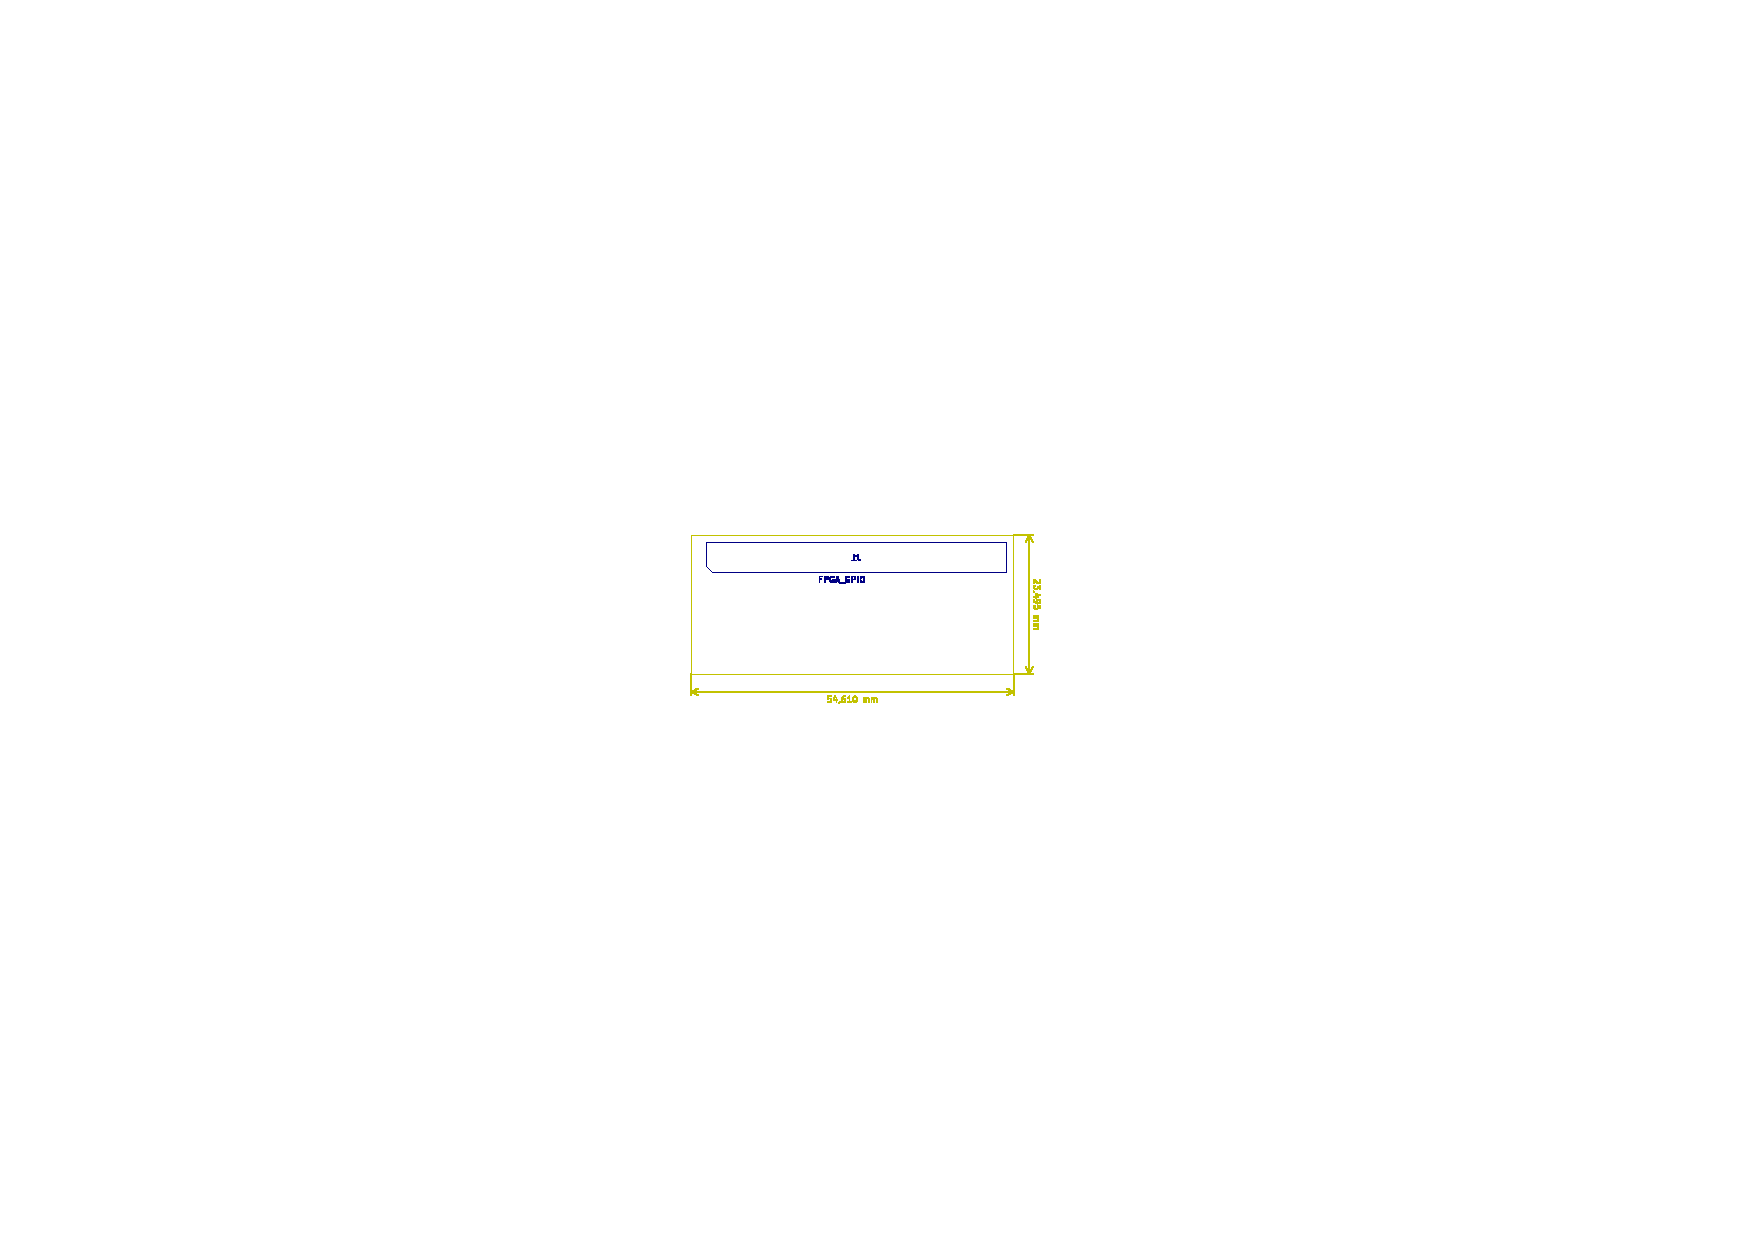
\includegraphics[width = 15cm]{SAUER/Grafiken/Prot1/BFAB.png}
\caption{Bestückungsplan Rückseite \& Bemaßung}
\label{Prot1_BFAB}
\end{center}
\end{figure}